\documentclass[12pt, letterpaper]{scrartcl}

\usepackage{fullpage} % Set margins and place page numbers at bottom center
\usepackage[shortlabels]{enumitem} % Use a. in the enumerate
\usepackage{amsmath} % aligned equations
\usepackage{graphicx} % include figure
\usepackage{float} % usage of H for figure float
%\usepackage{amssymb} % \blacksqure

\begin{document}

% ### Header - start ###
    \begin{center}
    	\hrule
    	\vspace{0.4cm}
    	{\textbf { {\large Homework 1} \\ EE 668 --- Information Theory}}
    \end{center}
    { \textbf{Name:} Ali Zafari \hspace{\fill} \textbf{Student Number:} 800350381 \hspace{\fill} \textbf{Fall 2022} } \newline\hrule
% ### Header - end ###

\paragraph*{Problem 1.1} \hfill
\begin{enumerate}[a.]
    \item The alphabet for random variable $X$ is:
        \begin{equation*}
            \mathcal{X}=\{1, 2, 3, ...\}
        \end{equation*}
        and its probability mass function (the coin is \textbf{fair}):
        \begin{equation*}
            P(X=x)={(\frac{1}{2}})^{x-1}\times\frac{1}{2}={(\frac{1}{2}})^{x}
        \end{equation*}
        Entropy is as follows:
        \begin{align*}
                H(X)&=-\sum_{x}P(x)\log P(x)=-\sum_{x=1}^{+\infty}{(\frac{1}{2}})^{x}\log{(\frac{1}{2}})^{x} \\
                    &=-\sum_{x=1}^{+\infty}x{(\frac{1}{2}})^{x}\\
                    &=\frac{\frac{1}{2}}{(1-\frac{1}{2})^2}\\
                    &=2
            \end{align*}
            
    \item With a fair coin ($p=\frac{1}{2}$), the best questions to be asked are the questions which have the highest information for guessing the value of $X$. First question should be "Is X equal to 1?". There is a chance of 50\% that we find out $X$ is zero. If not, then the next reasonable question would be "Is X equal to 2?". Even by having a No answer for this question, we are confident that we have removed uncertainty by 75\% about the value of X. By doing so, (on average) only 25\% of times we will be required to ask 3 or more questions to find the value of $X$. To calculate the average number of questions need to be asked to find the exact value of $X$ in this approach, we calculate the expected value of the number of questions as $\sum_{x=1}^{+\infty}x(\frac{1}{2})^x=2$. This value is equal to the entropy of the random variable.
\end{enumerate}
\hrule

\paragraph*{Problem 1.2} \hfill
\begin{enumerate}[a.]
    \item First we need to calculate the marginal distribution for both $X$ and $Y$.
    \begin{center}
        \begin{tabular}{c|cc}
        $X$    & 0             & 1             \\ \hline 
         \\[-1em]
        $P(X)$ & $\frac{1}{2}$ & $\frac{1}{2}$ \\
        \end{tabular}
        \qquad
        \begin{tabular}{c|cc}
        \textbf{$Y$}    & 0              & 1              \\ \hline
         \\[-1em]
        \textbf{$P(Y)$} & $\frac{5}{12}$ & $\frac{7}{12}$ \\
        \end{tabular}
    \end{center}
    
    The entropies can then be calculated as:
    \begin{align*}
        &H(X)=-\sum_{x} p(x)\log p(x)=1\\
        &H(Y)=-\sum_{y} p(y)\log p(y)=0.97987
    \end{align*}

    \item Conditional probabilities:
    \begin{center}
        \begin{tabular}{c|c|c}
            $P(X|Y)$    & $Y=0$             & $Y=1$        \\ \hline 
            &\\[-1em]
            $X=0$ & $\frac{3}{5}$ & $\frac{3}{7}$   \\ 
            &\\[-1em]
            \hline
            \\[-1em]
            $X=1$ & $\frac{2}{5}$ & $\frac{4}{7}$   \\
        \end{tabular}
        \qquad
        \begin{tabular}{c|c|c}
            $P(Y|X)$    & $Y=0$             & $Y=1$        \\ \hline 
            &\\[-1em]
            $X=0$ & $\frac{1}{2}$ & $\frac{1}{2}$   \\ 
            &\\[-1em]
            \hline
            \\[-1em]
            $X=1$ & $\frac{1}{3}$ & $\frac{2}{3}$   \\
        \end{tabular}
    \end{center}
    The conditional entropies are the expected value of the conditional probability over the joint entropy:
    \begin{align*}
        &H(X|Y)=-\sum_{y}\sum_{x} p(x,y)\log p(x|y)=0.97928\\
        &H(Y|X)=-\sum_{x}\sum_{y} p(x,y)\log p(y|x)=0.95915
    \end{align*}
    
    \item Venn diagram.
    \begin{align*}
        H(X,Y)=-\sum_{x}\sum_{y} p(x,y)\log p(x,y)=1.95915
    \end{align*}
    
    \item
    \begin{align*}
        H(Y)-H(Y|X)=0.97987-0.95915=0.02072
    \end{align*}
    
    \item
    \begin{align*}
        I(X;Y)=H(X)-H(X|Y)=1-0.97928=0.02072
    \end{align*}
    
    \item Venn diagram:
    \begin{figure}[H]
    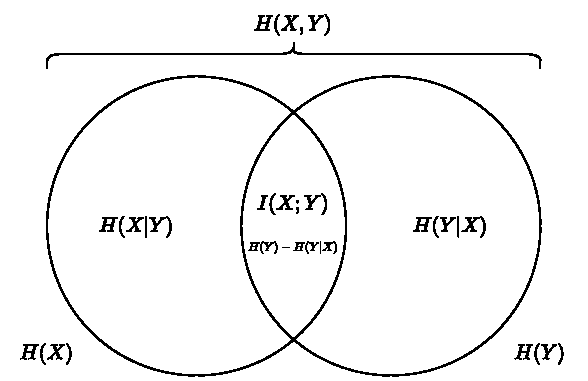
\includegraphics[width=0.6\linewidth]{hw1_figures/venn.pdf}
    \centering
    \caption{Venn Diagram of Information Measures of $X$ and $Y$}
    \end{figure}
\end{enumerate}
\hrule

\paragraph*{Problem 1.3} \hfill
\begin{align*}
    &H(p)=-\sum_{x} p(x)\log p(x)=1.5\\
    &H(q)=-\sum_{x} q(x)\log q(x)=1.5850\\\\
    &D(p||q)=\sum_{x} p(x)\log\frac{p(x)}{q(x)}=0.0849\\
    &D(q||p)=\sum_{x} q(x)\log\frac{q(x)}{p(x)}=0.0817
\end{align*}
Last two equations verify that $D(p||q)\neq D(q||p)$.
\newline\hrule

\paragraph*{Problem 1.4} \hfill\newline
Taylor series expansion of an infinitely differentiable function $f(x)$ at point $x=a$ is
\begin{align*}
    f(x)&=\sum_{n=0}^{+\infty}\frac{f^{(n)}}{n!}(x-a)^n\\
    &=f(a)+\frac{f^{(1)}(a)}{1!}(x-a)+\frac{f^{(2)}(a)}{2!}(x-a)^2+\frac{f^{(3)}(a)}{3!}(x-a)^3+\dots
\end{align*}
We now consider Taylor expansion of $\ln(x)$ at $x=1$:
\begin{align*}
    \ln(x)\bigg\rvert_{x=a}&=\ln(a)+\frac{1}{1!}\frac{1}{x}(x-a)+\frac{1}{2!}(-\frac{1}{x^2})(x-a)^2+\dots\\
    \ln(x)\bigg\rvert_{x=1}&=0+x-1-\frac{1}{2}(x-1)^2+\dots
\end{align*}
Since the term $-\frac{1}{2}(x-1)^2$ is always negative we can write:
\begin{align*}
    \ln(x)\leq x-1
\end{align*}
As $x>0$ we can use a change of variable as $y=\frac{1}{x}$ (noting that $y$ has a range of $y>0$ same as $x$):
    \begin{align*}
    \ln(\frac{1}{y})&\leq \frac{1}{y}-1\\
    -\ln(y)&\leq \frac{1}{y}-1\\
    \ln(y)&\geq 1-\frac{1}{y}
    \end{align*}
\hrule
\end{document}

